\documentclass[sigconf]{acmart}

\usepackage{booktabs} % For formal tables
\usepackage[inline]{enumitem}
\usepackage{indentfirst}

%% \name command
%% - allows break before /
\usepackage{etoolbox}
\usepackage{xstring}
\DeclareListParser{\doslashlist}{/}
\newcounter{ndnNameComponentCounter}%
\newcommand{\name}[1]{{%
  \setcounter{ndnNameComponentCounter}{0}%
  \renewcommand{\do}[1]{{%
    \ifnumgreater{\value{ndnNameComponentCounter}}{0}{\allowbreak/}{}%
    \ifnumodd{\value{ndnNameComponentCounter}}{}{}%
    \detokenize{##1}}%
    \stepcounter{ndnNameComponentCounter}}%
``{\fontfamily{cmtt}\small\selectfont\IfBeginWith{#1}{/}{/}{}\doslashlist{#1}}''%
}}

\newcommand{\TODO}[1]{\textcolor{red}{#1}}

\begin{document}
\title{NDN IoT Protocols on RIOT OS}

\author{Tianyuan Yu}
\affiliation{%
	\institution{Sichuan University}
}
\email{royu9710@outlook.com}

\author{Zhiyi Zhang}
\affiliation{%
  \institution{UCLA}
}
\email{zhiyi@cs.ucla.edu}

\begin{abstract}

The Named Data Networking (NDN) architecture provides simple solutions to the communication needs of Internet of Things (IoT) in terms of ease-of-use, security, and content delivery.
To utilize the desirable properties of NDN architecture in IoT scenarios, we are working to provide an integrated framework, dubbed NDNoT, to support IoT over NDN on RIOT OS, a friendly 
IoT operating system for constrained devices. NDNoT Protocols provides solutions to auto configuration, service discovery, data-centric security, content delivery, and other needs of IoT 
application developers. Utilizing NDN naming conventions, NDNoT aims to create an open environment where IoT applications and different services can easily cooperate and work together.
This report introduces the basic components of our framework and explains how these components function together. 
\end{abstract}

%Conference
\copyrightyear{} 
\acmYear{} 
\setcopyright{none}
\acmConference[]{}{}{}

\maketitle

\section{Introduction}

We argue that the Named Data Networking (NDN)~\cite{ndn-ccr} architecture provides simple solutions to the communication needs of the Internet of Things (IoT), for the following 5 reasons:
\begin{enumerate*} [label=(\roman*)]
	\item NDN builds the data-centric security into the network layer by securing data directly in a local network system instead of relying on secured sessions and trusted cloud servers.
	\item Naming conventions provide an open environment for applications and services to cooperate and function together.
	\item By naming data, NDN enables host multihoming and seamlessly utilizes all  communication interfaces (e.g., Bluetooth, BLE, Wi-Fi, 802.15.4).
	\item NDN natively supports content multicast and in-network caching.
	\item NDN provides a simple way of developing applications: developers focus on the data itself without worrying about DNS or IP configurations.
\end{enumerate*}

% Proposal
In this report, we introduce NDNoT on RIOT OS~\cite{baccelli2018riot}, an IoT framework running over the NDN architecture.
NDNoT uses semantic names as the centerpiece of the system: (consumer) applications use names to fetch named and secured content produced by other (producer) applications.
Compared to the existing IP-based IoT frameworks, NDNoT gets rid of the mapping (e.g., DNS, mDNS) between application-readable service identifiers (e,g., URI, service names) and network identifiers (e.g., IPv6 addresses).
Previously, we have NDN-RIOT~\cite{ndn-iot} package to provide basic NDN support on RIOT OS, we develop serveral modules upon the original NDN-RIOT, faciliting users to utilize application layer NDN protocols supports. 
We have been experimenting NDNoT framework on RIOT OS with Atmel SAM R21 Xpro boards.

\section{Application Scenario}

In a classic smart home application scenario, the home owner uses his Android phone or a Linux/macOS laptop as the controller to manage the IoT system.
With NDNoT, each IoT device (e.g., camera, temperature sensor, etc.) trusts the controller and is able to verify signatures generated by other IoT devices, so that the commands or content with fake or untrusted signatures will never be accepted.
Notably, the trust anchor (i.e., the controller certificate) is stored locally on the controller device instead of a remote cloud server.
All devices register their name prefixes for provided services and a device is able to discover the available services under other prefixes by fetching the metadata.
When data privacy is needed, the home owner can configure the access rights for each device/service in the system so that only authorized devices/services can access (i.e., decrypt) the private data.

\textbf{Assumptions:} We assume that devices in home network are in each other's one hop, at most two hops distance, since typical IEEE 802.15.4 can serve household enviornment well. This network allows direct commnunication within nodes or at most one relay/forwarder betweem them. 
Forwarder simply transponds packets under home prefix. 
At least one stable and reliable controller inside network can provide bootstrap or authentication service, managing identities and access permission. Before bootstrapping, devices don't have identities in the network. During bootstrapping, controller will assign proper identities for devices, 
in the form of trust anchor signed certificate. The trust anchor is manually pre-installed in the network. After bootstrapping, devices have their own communication keys, faciliting further inner communication inside home network and securing keys used in bootstrapping not leaked. 

\section{NDNoT Framework: A Top-Down View}

NDNoT devices are also able to communicate with Android phones and Linux or macOS devices that are running the NDN protocol stack.
In an IoT scenario, an Android phone or a Linux/macOS device can play the role of domain controller.

In this section, we provide a top-down view of the framework and explain how each module works.
%Basically, new coming device should bootstrap first in local NDN, fetching its certificate to explore further services in this scenario. After proper bootstrap and configuration of available services, device will be permitted to exchange data in local NDN. Schematized trust will also be assigned by domain controller to guarantee secure IoT networking.  

\subsection{Bootstrapping}

The bootstrapping module provides applications an automatic way of bootstrapping. This module is strictly required for new added devices to
\begin{enumerate*} [label=(\roman*)]
	\item communicate with other IoT devices,
	and
	\item build a trust relationship with the local IoT system and sign/verify NDN Data packets.
\end{enumerate*}

Based on a pre-shared secret (e.g., by scanning a QR code), the security bootstrapping enables an IoT device/application to
\begin{enumerate*} [label=(\roman*)]
	\item install the certificate of the controller as a trust anchor
	and
	\item obtain a certified name linked to a certificate signed by the controller.
\end{enumerate*}

A new device who want to join the network should have at least a pair of bootstrap key. At the beginning of bootstrapping, the 
new coming device broadcast a interest started with /ndn/sign-on, appended with the digest of BKpub, and a Diffie Hellman key bits.
In this part, to minimize the time consumed in bootstrapping, we use an variant key exchange algorithm from classic Diffie Hellman. 
The token in the interest name is assemblied from four sperate tokens, 64bits for each part. Although this break down in key bits 
will impair the strength of security, given that home network devices generally have lifetime shorter than several years, this tradeoff is reasonable. 

\begin{figure}[h]
	\vspace{-0.1cm}
	\centering
	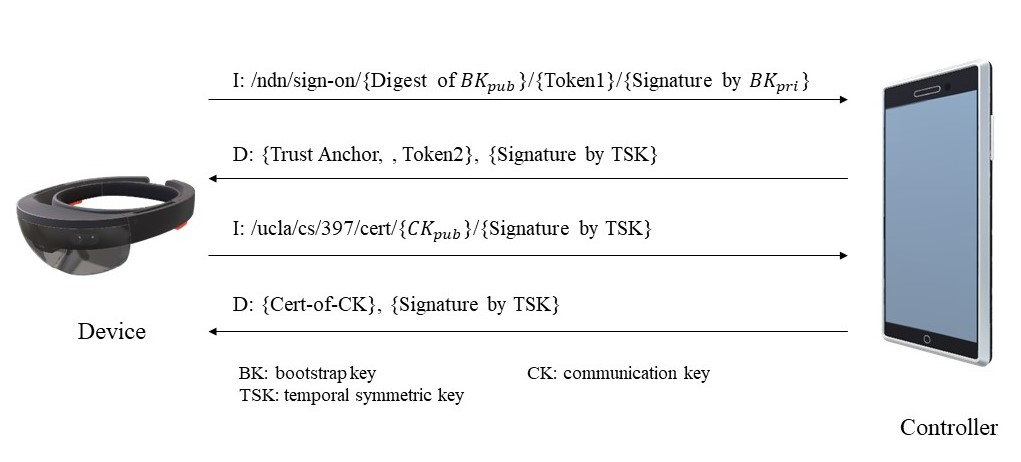
\includegraphics[width=0.45\textwidth]{figures/bootstrap}
	\caption{NDNoT Bootstrapping}
	\vspace{-0.1cm}
	\label{fig:bootstrap}
\end{figure}

Device signs this interest by BKpri and send the interest packet to IEEE 802.15.4 interface. When controller receives this bootstrapping request,
it firstly extract the digest of BKpub in the interest, and compare it with candidate BKpub keys pre-shared. If matched, the signature verification 
begins. Only a valid signature can lead controller's trust on the request sending device. Controller will then send back a bootstrap response, 
containing the a hash segment, indicating controller hold the pre-shared BKpub before the bootstrapping process, an anchor certificate, and four Diffie Hellman key 
bits parts. This data packet is signed by anchor key. 

After device verifying signature and installing the anchor certificate, two sides in bootstrapping build a trust. On this basis, device read home prefix from 
anchor certificate, and expresses a certificate interest under the namescope /\{home prefix\}/cert, appended with CKpub applied for in-network communication use. This interest 
is signed by HMAC key derived from the key exchange. Certificate request expects an anchor signed certificate from controller, inside which is identities allocated 
from bootstrapping controller. 

Basically, an anchor signed communication certificate is the end of bootstrapping, device can read identities and install commnuication certificates from the second round response. 
To devices who need identities dynamically, other than one-time allocated, a reverse "identity application" will use similar workflow with this one. Currently we don't support this yet.

\subsection{Service Discovery}

The service discovery module helps applications find available services in the local IoT network and also to advertise their own services to other nodes.
Running over NDN, the service discovery is implemented by prefix discovery and prefix registration.
Unlike the service discovery solutions in TCP/IP networks which are based on a (distributed) database query,
NDNoT on RIOT OS utilizes NDN's naming convention and the use of application names at the \emph{network layer} to facilitate the discovery/advertisement process.

To start service discovery, the device must be bootstrapped first, to obtain assigned identities and communication certificate inside the network.
This dependency is guaranteed by system design. two pre-processing steps are required to begin service discoery. 
\begin{enumerate*} [label=(\roman*)]
	\item device obtains identities and certificate from holder thread (e.g., lightweight NFD),
	and
	\item user provides served prefixes in this network.
\end{enumerate*}

After pre-processing, prefixes are aggregated to several service names, device will periodically broadcast service names 
along with corresponding identities names, in convention /\{home prefix\}/servicediscovery/\{identity\}/servicelist/\{service names\}. 
Time interval between two broadcast can be defined users, or set by default. To reduce communication overhead in constrained devices network, 
a longer interval is preferred, for most nodes in home network scenario being comparatively stationary and stable in their functionalities and positions.  

Other than periodically broadcast interest to notify neighbours the available identities and service names, discovery process also need devices
to listen other broadcast interests under the namescope /\{home prefix\}/servicediscovery, collecting available identities and service names around.

\begin{figure}[h]
	\vspace{-0.1cm}
	\centering
	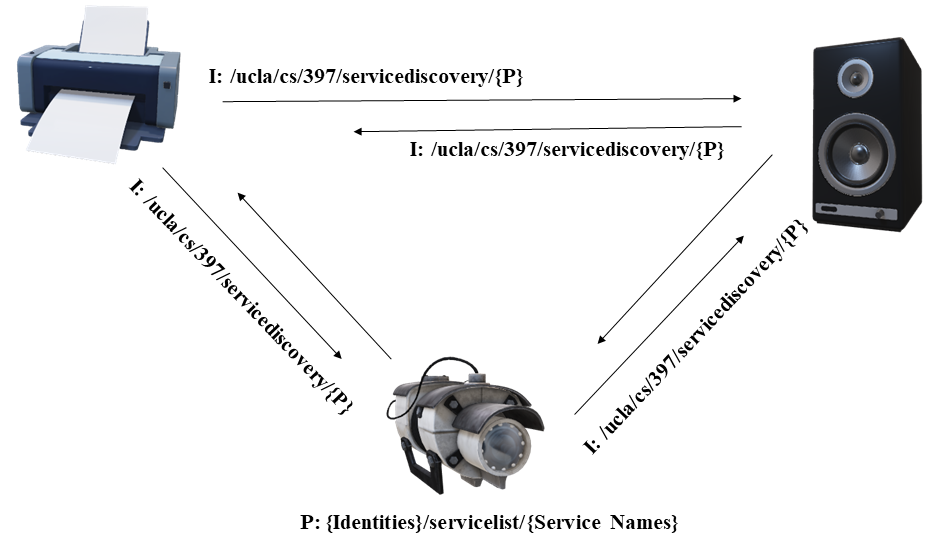
\includegraphics[width=0.45\textwidth]{figures/service-discovery}
	\caption{NDNoT Service Discovery Broadcast}
	\vspace{-0.1cm}
	\label{fig:servicediscovery-broadcast}
\end{figure}

When one want to know more about available services, beyond basic information. It can express a unicast query, which carry specific identity name and service name, 
targetting devices who serve certain prefixes, to ask detailed naming convnetion or parameters needed to apply for this service. An example interest can be 
/ucla/cs/397/sensor0001/query/readStatus, which means a bootstrapped device quering identity /sensor0001 detail information of service "readStatus". This query expect 
a metadata coming back from target identity.

\begin{figure}[h]
	\vspace{-0.1cm}
	\centering
	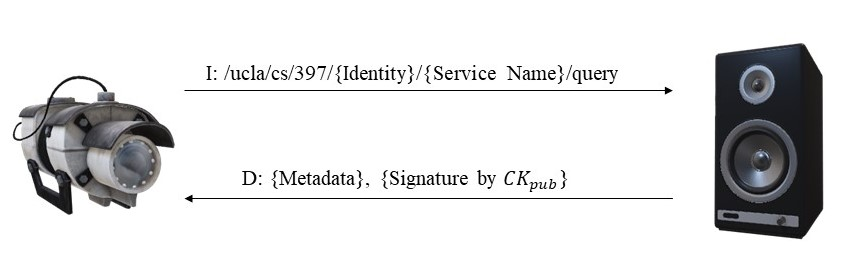
\includegraphics[width=0.45\textwidth]{figures/service-discovery-query}
	\caption{NDNoT Service Discovery Query}	\vspace{-0.1cm}
	\label{fig:servicediscovery-query}
\end{figure}

In IoT context, an important factor can't be ignored is energy consumption. constrained devices prohibit energy expensive operation, like RF communication, always online. 
Therefore, devices need to be in sleep mode from time to time, leading to a challenge of delicately tunning all devices awake in same time slots. However, the synchronization 
issue is beyond our discussion for now. 

\subsection{Access control}
IoT devices like smart home cameras and door locks require high data confidentiality and strict access control, which are supported by NDNoT's access control module.
Instead of storing the access keys in remote cloud servers, NDNoT provides localized access control, allowing the local user (e.g., home owner) to have complete control of the data produced and consumed by the IoT system.
By naming both digital keys and data, NDNoT automates the key distribution process of the access control scheme, thus minimizing manual configuration.
NDNoT on RIOT OS provide identities based access control and prefixes based access control as two options in our implementaion. 

\subsubsection{Identities Based Access Control}

One of major difficulties of deploying strong security system in IoT scenario is the limitation of computation resources. Crypographic operation will dominate constrained platforms' CPU if we frequently call those expensive 
functions. In fact, a device may serve many access control needed prefixes in a home network, making key management a big issue if simply using one-key-per-prefix method. Therefore, applying access control on identities, rather than 
certain prefixes is a candidate solution. In this method, a producer first communicate with authentication server, using classic Diffie Hellman key exchange algorithm based on ECDSA keys (ECDH), to generate a seed for content encryption.
Its access control request interest include identity name and Diffie Hellman key bits and a ECDSA signature by its communication key. As an optional parameter, a scheme of access condition may also 
be appended to the name, informing authentication server what type of consumers/applicants can have the decrytion key of the packets.

\begin{figure}[h]
	\vspace{-0.1cm}
	\centering
	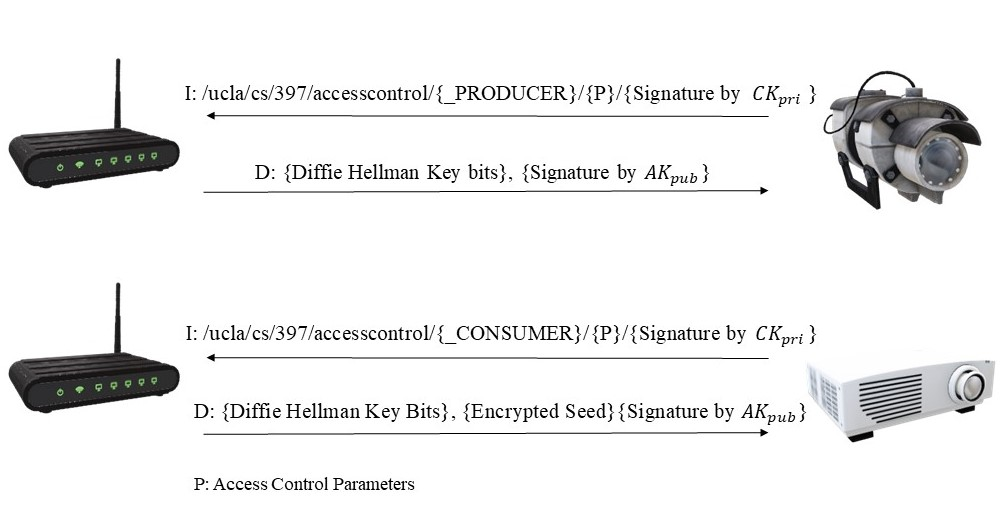
\includegraphics[width=0.45\textwidth]{figures/access-control}
	\caption{NDNoT Access Control}
	\vspace{-0.1cm}
	\label{fig:Access-Control}
\end{figure}

On the access application side, a consumer identity expresses a signed request, which includes the identity it want to get access to. This interst also may include an optional parameter to prove the request sender has the right of getting access. 
Successfully verifying the signature, authentication server will search the list of registered producer identities, and check access control scheme to decide whether to the applicant have the right to obtain the seed of desired producer identity. 
After that authentication server and access applicant will also use classic Diffie Hellman algorithm on ECDSA (ECDH) to decide the encryption key for transmitting producer's access seed on channel.

\subsubsection{Prefixes Based Access Control}
To devices who need precisely control the access of content, an identity based method isn't enough. As an alternative solution, we also provide access control on certain producer assigned prefixes. In this method, producer must name specific prefixes 
to authentication server. This solution uses similar workflow. 

\section{Current Status and Future Work}

RIOT OS currently provides support for Ethernet (used by emulator) and IEEE 802.15.4, thereby NDNoT Protocols can only run these two layer 2 protocols now.
Newest version bootstrapping still doesn't provide a tunnel for "identity application", since the design of bootstrapping itself keeps updating. Access Contorl 
for now only support identities based method. Although our network is at most two hops scenario, bootstrapping still need happen when controller and device can 
hear each other directly. Controller for now can only be a RIOT OS device, rather than NFD installed Android phone, because current NFD doesn't support IEEE 802.15.4 yet, 
and most cellphones don't have such network interface either. Raspberry Pi is a promising candidate, benefiting from IEEE 802.15.4 interface support and enough powerful hardware to run 
NFD. Adding support for 802.15.4 on NFD, we will easily deploy Raspberry Pi as a strong gateway router, serving both bootrapping and authentication in home 
network. Memory problems still exist in runtime, package occupying too much space. Compared to similar application layer protocol CoAP's implementation 
on RIOT OS, which has similar memory usage number with us, a potential solution is not to enable all modules on a single device (e.g., a camera may not need to know other's 
services all the time, but need strict access control when online). Future work will cover filling extra functionalities and fixing memory usage problem. 

\bibliographystyle{plain}
\bibliography{ndn}

\end{document}
